\documentclass{article}
\usepackage{graphicx}
\usepackage[left=1in, right=1in, top=1in, bottom=1in]{geometry}
\begin{document}

\section*{Editors}

Thanks to the editors for the opportunity to revise and resubmit the previous version of the manuscript. I have attended to all of yours and the reviewers's recommendations for revision, and I believe the result is a stronger, clearer, and potentially more impactful manuscript. Here I note my responses to the editors' suggestions, more detailed responses to the reviewer suggestions follow below.

\subsection*{Major Points}
\begin{itemize}
    \item Regarding errors in the Southern Women data matrix, these are now fixed, and the data analyzed are the canonical data set. See response to Reviewer 1 below.
    \item I also addressed R1's insightful point about the differences between odd and even iterations with regard to their correlation with the Bonacich centrality; see response to the reviewer below. 
    \item Regarding R2's call for a more effective statement of the novelty of the argument and key contributions, see various responses to the reviewer's suggestions below, which I took seriously and became the basis of a thorough rewrite of the manuscript. 
    \item With regard to broadening the coverage of the work, I have added a section on previous work as background (section 2). This version of the paper now incorporates Everett and Borgatti's 2013 piece throughout, and reframes CA (and Bonacich centrality analysis) as options within the ``dual projection'' framework they outline in that article, while making new connections between higher order axes in the Bonacich decomposition and their proposed approach to finding sets of structurally equivalent actors in two-mode networks. 
    \item With regard to strengthening the linkages between the paper's argument and Breiger's duality idea, see the response to R2's suggestions below. 
\end{itemize}

\subsection*{Minor Points}
\begin{itemize}
    \item - \underline{Editors}: \textit{p. 4 of ``the sum of the q-1 centralities'' is a little confusing. If we correctly understand your point, q-1 refers to the iteration rather than how many centralities are being summed. Perhaps this could be that could be reworded.''} \textbf{Response}: The relevant passage has been reworded to improve clarity and accuracy. 
    \item -  \underline{Editors}: \textit{Notation in eq. 19 and 20 seems slightly awkward - the left-hand side should somehow show that those are the transformed values, not the same as on the right-hand side (which currently is written the same way).} \textbf{Response}: I have added a single apostrophe (prime) symbol to indicate that the left hand side quantity is a transformed value.
    \item - \underline{Editors}: \textit{For eq. 21 and 22, it might be helpful to note how the eigenanalysis of the two product matrices relates to the SVD of the original.} \textbf{Response}: I have added some wording noting the links between eq. 21 and 22 and eq. 9 and 10.
\end{itemize}

\newpage
\section*{Reviewer 1}

\noindent\textbf{State key points and conclusions at the beginning}\newline
\textit{Response}: Thanks for this comment. Given the newly added material, I streamlined the introduction in this version of the paper. However, the introductory paragraphs have been rewritten to highlight the key points and conclusions, which are also summarized in the rewritten abstract and highlights. \newline

\noindent\textbf{Add distinction between Bonacich and CA to the highlights}\newline
\textit{Response}: Thanks for this suggestion. I have now included a relevant highlight bullet point noting the relevant analytic contrast of Bonacich versus CA. \newline

\noindent\textbf{Data errors in the Southern Women two-mode matrix}\newline
\textit{Response}: Thanks for calling attention to this---rather embarrassing---error; it's definitely a cautionary tale against manually copying data. I have corrected the data, and as you can see in the analysis file included as supplementary material, I now extract the Southern Women data directly from the \texttt{networkdata} package.\footnote{\texttt{https://www.rdocumentation.org/packages/networkdata/versions/0.1.6}} My table now matches those in the references you mentioned exactly. Note, however, that while you are correct that Frances, Eleanor, and Ruth did not attend E4, Nora did not attend E8, at least according to the published tables in Doreian et al (2004), Kovacs (2010), and the Figure 1 from Freeman (2003), shown above; in these papers, as you can see, Nora's event set is \{E6, E7, E9, E10, E11, E12, E13, E14\}. I think the confusion comes from the fact that Freeman used a non-chronological order of events (as is evident from the date labels in the figure) that emphasizes the group structure of the women. This non-chronological ordering leads to a different labeling of events than when events are arranged in chronological order; this is the ordering of events used by Doreian et al. 2004 and Kovacs (2010). In this event labeling, Nora does not attend E8 (the event that took place on 9/16.) However, note that this is obviously \textit{not} the ordering of events in the original Breiger (1974)---nor for that matter the earlier Doreian (1979) piece in \textit{Social Networks} that used Q-Analysis. In this \textit{chronological} labeling of events, Nora does attend ``E8" (the event that took place on 5/19), as evident in Breiger (1974, p. 186, fig. 2a). In any case, to forestall any confusion, and given that, in the \texttt{networkdata} package, the columns of the biadjacency matrix corresponding to the \texttt{southern\_women} object containing the Southern Women data come ordered using the Freeman (2003) ordering, I'm sticking to the non-chronological event labeling. I now include a brief discussion in the paper clarifying this issue.\newline 


\begin{figure}
    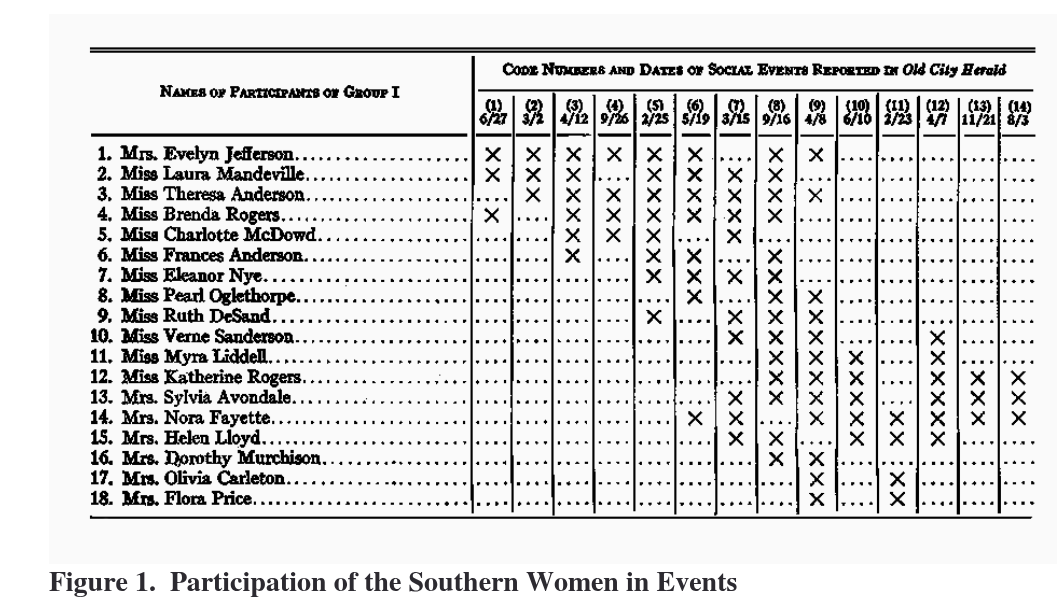
\includegraphics[width=1.0\textwidth]{Reviews and Response/sw-original.png}
\end{figure}


\noindent\textbf{Appropriateness of the term ``reflective centrality''}\newline
\textit{Response}: Thanks for this comment, which I thought was very helpful. The term centrality introduces a level of conceptual imprecision that is best avoided. I liked your suggestion of using the more neutral term ``scores'' instead, which I implemented throughout the paper.\newline

\noindent\textbf{Differences between odd and even iterations}\newline
\underline{Reviewer}: \textit{What complicates things, as you know, is the difference between odd and even iterations of the reflective algorithm (see your comments in the first paragraph on p. 4, as well as comments of H \& H). One point you might consider adding is that, for the first even iterations (iterations 2, 4, 6, 8, and 10), the magnitude (absolute value) of the correlation of reflected scores with Bonacich centrality (for persons, and for groups) tends to increase with subsequent iterations (and, in the limit, is .682 for persons by iteration 40 for persons), whereas, for the first odd iterations (iterations 3, 5, 7, 9, 11), the magnitude of the correlation decreases (toward a limiting value, once again, of .682 by iteration 41). Can you relate this to the differences between odd and even iterations that you (and H\&H) discuss?}

\noindent\textit{Response}: Thanks for this very insightful observation. I think that indeed there is a link between how the even and odd iterations are defined mathematically and their different patterns of correlations with the Bonacich centrality. Indeed, the early definitions of the odd iterations are closest to Bonacich's dual centrality idea, whereby people are central if they belong to central groups (and the centrality of groups is a function of the centrality of people who belong to them), which explains why we see a stronger correlation between the third reflection and Bonacich centrality which attenuates to the equilibrium value after higher reflections, and a lower correlation between the second iteration and the same quantity, which increases to the same value as the two rankings converge. This is now noted and explained in footnote 9 of the main text, along with an acknowledgment. Note, however, that I get a different value than you for the equilibrium correlation (see attached replication materials). \newline

\noindent\textbf{Missed connection between Bonacich and CA regarding ``groupiness''}\newline
\textit{Response}: Thanks very much for raising this point, which made me think about and consider issues that I missed in the first version of the paper. You are right that the second dimension of the Bonacich centrality reveals a dimension of ``groupiness'' in the data; however, this dimension is not quite the same as that of CA. In fact, it became clear to me that what it reveals are continuous approximations to structural equivalence in the data, which makes sense if, indeed, the CA scores are continuous approximations to a regular equivalence style criterion (or generalized relational similarity). We can check this claim by comparing the blocking obtained from the second Bonacich dimension and that produced by Everett and Borgatti (2013, Table 5) using a proportion-matching criterion for structural equivalence, and see that they agree quite closely, a discussion that I now include in the paper. The groupings in the second Bonacich dimension end up being secondary core-periphery partitions, net of the main one. This reinforces my previous claim, which was poorly argued for in the previous version of the paper, that the Bonacich decomposition comes closer to reproducing the original ``input data'' than the CA decomposition. \newline

\noindent\textbf{Reversing column ordering on some figures}\newline
\textit{Response}: Thanks for this suggestion. I have re-plotted the figures using the suggested column ordering. \newline

\noindent\textbf{Confusing equations}\newline
\underline{Reviewer}: \textit{What confused me about eqs. (23) and (24) is that I don't think the (respective) expressions in parentheses are symmetric matrices, and so I don't see how to take an eigenvector. (Each of the rows, but not the columns, sum to 1.)}

\noindent \textit{Response}: Thanks for this observation. You are correct that I did not adequately explain where the eigenvectors corresponding to the CA (and HH) scores come from. You are right that the equations result in row-stochastic matrices (row sums equal 1.0) that are square but not symmetric. You can still do a spectral decomposition of each of these matrices, but the first (dominant) eigenvalue will be 1.0, and the associated eigenvectors will be filled with constant values. So the relevant eigenvector we seek, which is the first CA dimension, is that associated with the \textit{second} largest eigenvalue, and the second CA dimension is that associated with the third, and so forth. Another way of saying it is that we can perform the usual eigendecomposition of the row-stochastic projection matrices, discard the first trivial eigenvalue and eigenvector and treat the second as the first, the third as the second, etc., and that will be equivalent to the CA solution, the same scores that simple CA of the original rectangular Affiliation matrix would yield (but note that we run into a similar situation when computing CA via SVD of the row and column mass normalized affiliation matrix, which results in a solution with a first eigenvalue of 1.0 and associated trivial eigenvectors with person and event scores proportional to the row and column masses, which need to be discarded with the focus being on the second, third, eigenvalues and eigenvectors as Faust 2005, p. 126 notes). The relevant section of the paper has been rewritten to clarify these issues.\newline

\noindent\textbf{Confusing labeling of figures across multiple panels}\newline
\textit{Response}: I have re-rendered the figures so that the labeling is clearer. \newline

\noindent\textbf{Missing Freeman citation}\newline
\textit{Response}: Freeman citation is now added and discussed in the paper. \newline

\newpage
\section*{Reviewer 2}

\textbf{Insufficient engagement with Breiger's duality idea}\newline
\textit{Response}: Thanks for this comment, which proved pivotal in my revision efforts for this draft. In this version of the paper, I have endeavored to make the linkages between CA, Bonacich centrality analysis, and duality clearer in the text. I have also incorporated a more in-depth discussion of Everett and Borgatti's dual projection approach, and re-framed both CA and centrality analysis as two distinct but related options within that wider framework, which also helps to make the link to the duality notion crisper. \newline

\noindent\textbf{More extensive introduction and background}\newline
\textit{Response}: Thanks also for this comment, which informed most of the new material that has been added to this version of the paper, particularly the new section 2. I believe that with this background in hand, the paper's arguments and contribution can be more clearly stated and appreciated. \newline

\noindent\textbf{More even-handed consideration of the visualization aspects of the CA/MCA}\newline
\textit{Response}: Thanks for this comment, which made me realize that perhaps my previous comments regarding the focus on visualization on previous uses of CA and MCA for two-mode network analysis were coming off as overly dismissive. I have tried to rewrite the relevant sections in this draft to remove these connotations. My key point was more in reference to Borgatti and Everett's original 1997 piece, which seemed to think of CA primarily as a visualization tool, but was ignoring its usefulness for other network-analytic tasks such as clustering and ``a posteriori blockmodeling'' (in Wasserman and Anderson's terms). I hope that these points come out clearer in this version of the paper.  \newline

\noindent\textbf{Concerns over the interpretation of CA biplot distances}\newline
\textit{Response}: Thanks for this comment. In this version of the paper I provide a more in-depth discussion of what the inter-point distances in the usual CA correspondence plot get at. The rewritten section now ties the correspondence plot distances directly to the information in the degree-adjusted projection matrices, which leads to a more straightforward interpretation of the CA correspondence plot as a low-rank representation of the degree-adjusted proximity matrix, which makes the contrast to the Bonacich ``correspondence plot'' also clearer. \newline

\noindent\textbf{Insufficient discussion of positional equivalence and other blockmodeling approaches}\newline
\textit{Response}: Thanks for this comment, which I took to heart in rewriting key portions of the paper. As you can see, I contrasted different conceptions of positional equivalence (e.g., structural versus regular) central to my contrast between what CA does versus what the Bonacich decomposition does, also drawing on some of the literature that you suggested I look at (particularly D'Esposito et al's 2014 piece the contrast between CA and MCA distances), and previous work by Everett and Borgatti. While I did not engage in a full-on review of previous work on positional analyses of two-mode networks for reasons of relevance and space, the emphasis on the usefulness of CA for positional analysis (e.g., aka, ``spectral clustering'' in other fields) is evident throughout. Note that in the different flavors of blockmodeling, CA (or even Bonacich centrality) is closer to indirect or ``a posteriori'' blockmodeling (e.g., data-driven rather than model-driven) so the emphasis is different from optimization-based methods like Doreian, Batagelj, and Ferligoj's direct blockmodeling approach. Hopefully, what is new in the current approach relative to this previous work can be more clearly appreciated in this draft. \newline

\noindent\textbf{Insufficient discussion of other CA-based analytic strategies}\newline
\textit{Response}: Thanks for the reference to D’Ambrosio et al's work, which I read with great interest. In the end, when crafting the new background section, I realized that I couldn't cover all previous uses of CA and related techniques for two-mode network analysis. As a result, I decided to just focus on previous work that dealt with the simple-CA of the affiliation matrix, since that's what the core discussion of the paper is relevant for. However, I do note that this previous work focuses on MCA and related techniques (which your reference led me to) in various footnotes. \newline

\noindent\textbf{Better highlights section}\newline
\textit{Response}: Thanks for this comment, which along with a similar observation by the other review informed by revision of the highlights section. \newline

\noindent\textbf{Unclear figure}\newline
\textit{Response}: I have redone the old Figure 3 to remove any remaining confusion. \newline

\end{document}



